\documentclass{article}
\usepackage{polski}
\usepackage[T1]{fontenc}
\usepackage[utf8x]{inputenc}
\usepackage{booktabs}
\usepackage{multirow}
\usepackage{graphicx}
\usepackage{textcomp}
\usepackage{eurosym}
\usepackage{float}
\usepackage{adjustbox}
\usepackage{graphics}
\usepackage{tabularx}
\usepackage{rotating}
\usepackage{tabulary}
\usepackage{listings}
\usepackage{amstext}
\usepackage{xcolor}
\usepackage{url,textcomp}
\usepackage{amssymb}


\title{SCR- sieci komputerowe - Laboratorium - Raport 1}

\author{Damian Ryś}

 
\begin{document}

\maketitle


\tableofcontents
\section{Wstęp}
\hspace*{0.5cm}Grupa lab: E12-93c

Termin zajęć: CZW 15:15-16:55

Numer indeksu: 252936

Prowadzący: Dr inż. Jerzy Greblicki 
\section{Podstawowe komendy systemu Linux}
Do jedynych z najczęściej używanych poleceń podczas pracy z systemem Linux jest:
\begin{itemize}
    \item id - identyfikacja użytkownika
    \item passwd - zmiana hasła użytkownika
    \item who - informacje dotyczące bieżacej sesji
    \item cd - zmiana bieżącego katalogu na katalog będący argumentem polecenia
    \item mkdir - utworzenie nowego katalogu
    \item ls - wyświetlenie zawartości katalogu
    \item chmod - zmiana praw dostępu do pliku lub katalogu
    \item adduser - dodanie nowego użytkownika
\end{itemize}

\section{Instalacja Vim'a}
Zaczynamy od zaaktualizowania naszych pakietów przy użyciu
komendy \textit{sudo apt update}

\begin{figure}[H]
    \centering
    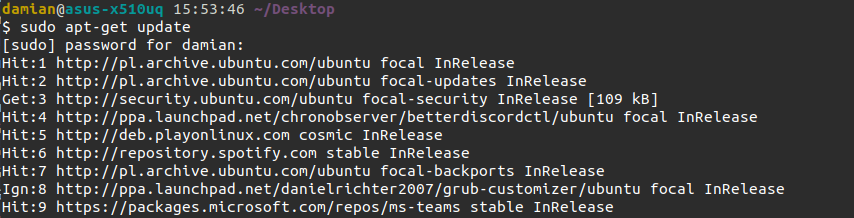
\includegraphics[totalheight=3cm]{data/sudoUpdate.png}
    \caption{Zaktualizowanie pakietów }
    \label{2}
\end{figure}

Dopiero teraz jesteśmy w stanie poprawnie zainstalować edytor
tekstu przy użyciu komendy \textit{sudo apt install vim}

\begin{figure}[H]
    \centering
    
    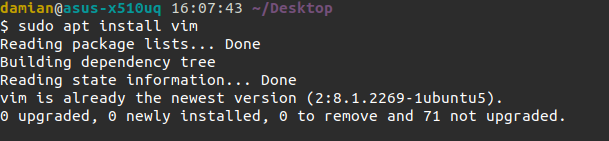
\includegraphics[totalheight=3cm]{data/installVim.png}
    \caption{Instalacja vima}
    \label{2}
\end{figure}


\section{Dodawanie użytkownika}
Naszego użytkownika możemy dodać przy pomocy komendy 
\textit{sudo adduser \textbf{nazwa użytkownika}}, w naszym przypadku będzie to 
użytkownik \textbf{Adam}.

\begin{figure}[H]
    \centering
    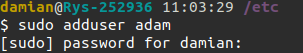
\includegraphics[totalheight=2cm]{data/userAdd.png}
    \caption{Instalacja vima}
    \label{2}
\end{figure}
Musimy tutaj następnie podać hasło użytkownika oraz potwierdzić je.
Takie konto jest widoczne w  \textbackslash etc\textbackslash Users 

\begin{figure}[H]
    \centering
    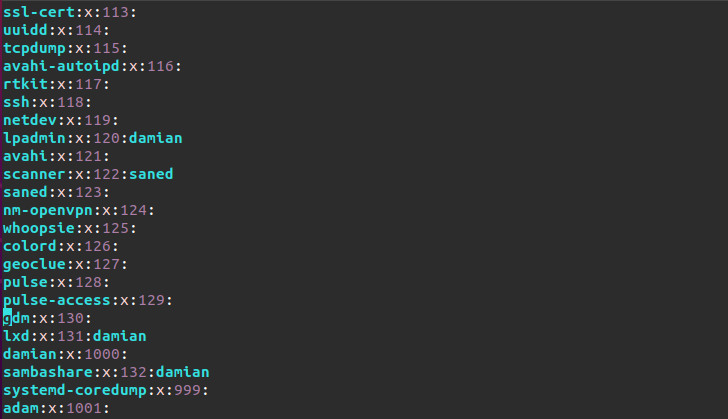
\includegraphics[totalheight=7cm]{data/AdamAddD.png}
    \caption{Lista użytkowników}
    \label{2}
\end{figure}


\section{Utworzenie nowej grupy i dodawanie użytkownika do grupy}
W celu utworzenia nowej grupy musimy skorzystać z polecenia \textit{group add \textbf{nazwa grupy}}
Tworzymy zatem grupe \textbf{studenci}
\begin{figure}[H]
    \centering
   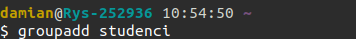
\includegraphics[totalheight=1cm]{data/addStudenci.png}
    \caption{Dodanie grupy studenci}
    \label{2}
\end{figure}
Następnie przy pomocy Vim wyświetlamy \textbackslash etc\textbackslash Grups i 
dodajemy ręcznie naszych użytkowników do grupy czego wynikiem jest:

\begin{figure}[H]
    \centering
   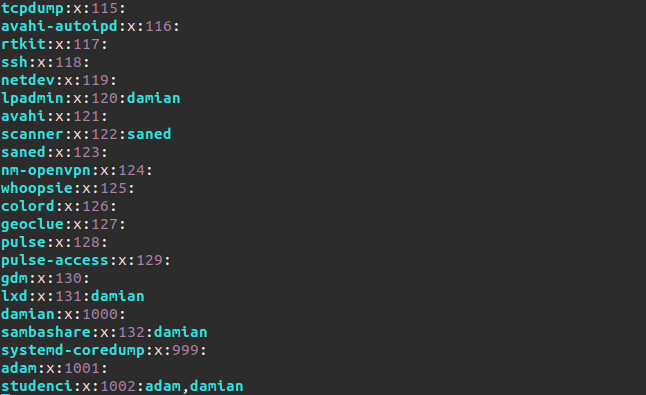
\includegraphics[totalheight=8cm]{data/gruupsWith.png}
    \caption{Użytkownicy w grupach}
    \label{2}
\end{figure}


\section{Komenda ls -la}
Przy pomocy komendy \textit{ls} jesteśmy w stanie wyświetlić w wyświetlić
cały nasz katalog z zawierającymi go plikami, natomiast dodatkowego
argumenty \textit{-la} powodują wyświetlenie również domyślnie ukrytych
plików oraz wyświetlenie dodatkowych informacji jak na przykład: 
\begin{itemize}
    \item prawa dostępu
    \item data modyfikacji
    \item rozmiar pliku
\end{itemize}


\begin{figure}[H]
    \centering
    \hspace*{-1cm}
    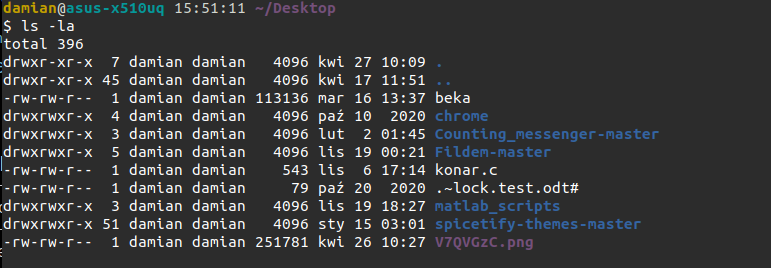
\includegraphics[totalheight=4cm]{data/ls-la.png}
    \caption{Komenda "ls -la"}
    \label{2}
\end{figure}



\section{Polecenie \emph{\textit{chmod}}}
Każdy plik oraz folder ma przypisane określone prawa dostępu dla różnych użytkowników systemu.\par
Polecenie \emph{\textbf{chmod}} zmienia parametry zezwolenia dostępu do plików w systemie Ubuntu.
Parametry polecenia chmod:
\emph{\textbf{chmod [opcje] uprawnienia plik}}\\

Uprawnienia jakie można nadać plikom:
\begin{itemize}
    \item \emph{\textbf{r}} - odczyt
    \item \emph{\textbf{w}} - zapis
    \item \emph{\textbf{x}} - wykonanie
\end{itemize}

Opis "klas" użytkowników, którym można zmienić uprawnienia:
\begin{itemize}
    \item  \emph{\textbf{user}} - właściciel
    \item  \emph{\textbf{group}} - grupa
    \item  \emph{\textbf{a}} - wszyscy użytkownicy
\end{itemize}
\subsection{Przykład na grupach}
Tworzę nowy folder testowy przy pomocy komendy \textit{mkdir} o nazwie
\textbf{test} i zmieniam jego uprawnienia na chmod 700, tzn że tylko 
główny użytkownik z permisjami będzie miał do niego dostęp. Do folderu nie da
się dostać czy zmodyfikować nazwy.
\begin{figure}[H]
    \centering
    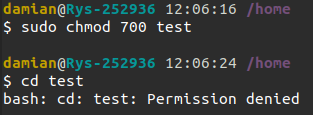
\includegraphics[totalheight=3cm]{data/chmod.png}
    \caption{Brak uprawnień }
    \label{2}
\end{figure}
Po nadaniu uprawnien dla użytkownika \textbf{damian} jesteśmy w stanie dokonywać zmian an pliku
\begin{figure}[H]
    \centering
    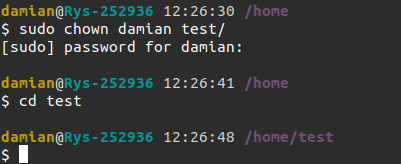
\includegraphics[totalheight=3cm]{data/chmod1.png}
    \caption{Nadane uprawnienia }
    \label{2}
\end{figure}
W kolejnym przykładzie chce pokazać ten wpływ również na grupy, po zmianie
konta użytkownika nie posiadam uprawnień, więc zmieniam uprawnienia nadaniu
\textit{chmod 770} oraz dodaje grupe \textbf{studenci} do tego folderu przy pomocy
\textit{chgrp studenci test}. Przelogowuje się na inne konto użytkownika i mogę zauważyć, że
posiadam wszelkie uprawnienia.

\begin{figure}[H]
    \centering
    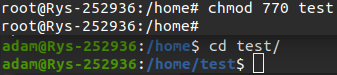
\includegraphics[totalheight=3cm]{data/chmod3.png}
    \caption{Nadane uprawnienia dla grupy studenci}
    \label{2}
\end{figure}


\end{document}